\chapter{Artificial Intelligence (AI) \cite{aci-1}}

\begin{enumerate}[itemsep=0.2cm]
    \item The field of artificial intelligence, or AI, attempts not just to understand but also to build intelligent entities. 

    \item \textbf{Acting humanly}: \textit{Turing test}
    \begin{enumerate}
        \item The \textbf{Turing Test}\indexlabel{Turing Test}, proposed by Alan Turing (1950), was designed to provide a satisfactory operational definition of intelligence.\\
        A computer passes the test if a human interrogator, after posing some written questions, cannot tell whether the written responses come from a person or from a computer.\\
        total Turing Test includes a video signal so that the interrogator can test the subject’s perceptual abilities, as well as the opportunity for the interrogator to pass physical objects “through the hatch.”\\
        To pass the total Turing Test, the computer will need:
        \begin{enumerate}
            \item \textbf{computer vision} to perceive objects

            \item \textbf{robotics} to manipulate objects and move about
        \end{enumerate}

        \item The computer would need to possess the following capabilities: 
        \begin{enumerate}
            \item \textbf{natural language processing} to enable it to communicate successfully in English

            \item \textbf{knowledge representation} to store what it knows or hears

            \item \textbf{automated reasoning} to use the stored information to answer questions and to draw new conclusions

            \item \textbf{machine learning} to adapt to new circumstances and to detect and extrapolate patterns
        \end{enumerate}
    \end{enumerate}

    \item \textbf{Thinking humanly}: \textit{The cognitive modeling approach} 
    \begin{enumerate}
        \item The interdisciplinary field of \textbf{cognitive science}\indexlabel{cognitive science} brings together computer models from AI and experimental techniques from psychology to construct precise and testable theories of the human mind. 

        \item an algorithm performs well on a task and that it is therefore a good model of human performance, or vice versa.
    \end{enumerate}

    \item \textbf{Thinking rationally}: \textit{The “laws of thought” approach}
    \begin{enumerate}
        \item The Greek philosopher Aristotle was one of the first to attempt to codify “right thinking,” that is, irrefutable reasoning processes

        \item His syllogisms/ arguments provided patterns for argument structures that always yielded correct conclusions when given correct premises-for example, \textit{“Socrates is a man; all men are mortal; therefore, Socrates is mortal.”}

        \item logicist tradition within artificial intelligence hopes to build on such programs to create intelligent systems. \\
        There are two main obstacles to this approach.
        \begin{enumerate}
            \item it is not easy to take informal knowledge and state it in the formal terms required by logical notation, particularly when the knowledge is less than 100\% certain

            \item there is a big difference between solving a problem “in principle” and solving it in practice.
        \end{enumerate}
    \end{enumerate}

    \item \textbf{Acting rationally}: \textit{The rational agent approach}
    \begin{enumerate}
        \item An \textbf{agent}\indexlabel{agent} is just something that acts (agent comes from the Latin agere, to do).\\
        Of course, all computer programs do something, but computer agents are expected to do more: operate autonomously, perceive their environment, persist over a prolonged time period, adapt to change, and create and pursue goals. 
        
        \item A \textbf{rational agent}\indexlabel{rational agent} is one that acts so as to achieve the best outcome or, when there is uncertainty, the best expected outcome.

        \item In the \textit{“laws of thought” approach} to AI, the emphasis was on correct inferences.\\
        Making correct inferences is sometimes part of being a rational agent, because one way to act rationally is to reason logically to the conclusion that a given action will achieve one’s goals and then to act on that conclusion.\\
        On the other hand, correct inference is not all of ration-ality; in some situations, there is no provably correct thing to do, but something must still be done.\\
        There are also ways of acting rationally that cannot be said to involve inference.\\
        \textbf{For example}, recoiling from a hot stove is a reflex action that is usually more successful than a slower action taken after careful deliberation.

        \item The rational-agent approach has two advantages over the other approaches. 
        \begin{enumerate}
            \item it is more general than the “laws of thought” approach because correct inference is just one of several possible mechanisms for achieving rationality. 

            \item it is more amenable to scientific development than are approaches based on human behavior or human thought. 
        \end{enumerate}

        \item The standard of rationality is mathematically well defined and completely general, and can be “unpacked” to generate agent designs that provably achieve it.\\
        Human behavior, on the other hand, is well adapted for one specific environment and is defined by, well, the sum total of all the things that humans do.

        \item \textbf{limited rationality}\indexlabel{limited rationality} - acting appropriately when there is not enough time to do all the computations one might like.
    \end{enumerate}
\end{enumerate}

\section{Fundamentals of AI \cite{aci-1}}

\subsection{Philosophy}
\begin{enumerate}
    \item \textbf{rationalism}\indexlabel{rationalism} Descartes was a strong advocate of the power of reasoning in understanding the world, a philosophy now called rationalism, and one that counts Aristotle and Leibnitz as members. 

    \item \textbf{dualism}\indexlabel{dualism}: Descartes was also a proponent of dualism.\\
    He held that there is a part of the human mind (or soul or spirit) that is outside of nature, exempt from physical laws.\\
    Animals, on the other hand, did not possess this dual quality; they could be treated as machines.

    \item \textbf{materialism}\indexlabel{materialism}: An alternative to dualism is materialism, which holds that the brain’s operation according to the laws of physics constitutes the mind.\\
    Free will is simply the way that the perception of available choices appears to the choosing entity.

    \item \textbf{empiricism}\indexlabel{empiricism}: the theory that all knowledge is based on experience derived from the senses.

    \item \textbf{induction}\indexlabel{induction}: that general rules are acquired by exposure to repeated associations between their elements.

    \item \textbf{logical positivism}\indexlabel{logical positivism}: holds that all knowledge can be characterized by logical theories connected

    \item \textbf{confirmation theory}\indexlabel{confirmation theory}: to analyze the acquisition of knowledge from experience

    \item the mind is the connection between knowledge and action

    \item because intelligence requires action as well as reasoning

    \item only by understanding how actions are justified can we understand how to build an agent whose actions are justifiable (or rational)
\end{enumerate}

\subsection{Mathematics}
\begin{enumerate}
    \item leap to a formal science required a level of mathematical formalization in three fundamental areas: logic, computation, and probability.

    \subsubsection*{Logic}

    \item The idea of formal logic can be traced back to the philosophers of \textbf{ancient Greece} who worked out the details of propositional, or Boolean logic.

    \item In 1879, \textbf{Gottlob Frege} (1848–1925) extended Boole’s logic to include objects and relations, creating the \textit{first-order logic}\\
    first-order logic could \textbf{not} capture the principle of mathematical induction needed to characterize the natural numbers.

    \item \textbf{Alfred Tarski} (1902–1983) introduced a theory of reference that shows how to relate the objects in a logic to objects in the real world.

    \item \textbf{algorithm}: a process or set of rules to be followed in calculations or other problem-solving operations, especially by a computer.\\
    The first nontrivial algorithm is thought to be Euclid’s algorithm for computing greatest common divisors.

    \item In 1931, Godel showed that limits on deduction do exist.\\
    His \textbf{incompleteness theorem}\indexlabel{incompleteness theorem} showed that in any formal theory as strong as Peano arithmetic (the elementary theory of natural numbers), there are true statements that are undecidable in the sense that they have no proof within the theory. \\
    some functions on the integers cannot be represented by an algorithm - that is, they cannot be computed. \\
    the notion of a computation or effective procedure really cannot be given a formal definition

    \subsubsection*{Computation}

    \item \textbf{Church–Turing thesis}\indexlabel{Church–Turing thesis}, which states that the Turing machine (Turing, 1936) is capable of computing any computable function, is generally accepted as providing a sufficient definition.\\
    Turing also showed that there were some functions that no Turing machine can compute.\\
    \textbf{For example}, no machine can tell in general whether a given program will return an answer on a given input or run forever. 

    \item a problem is called \textbf{intractable} if the time required to solve instances of the problem grows exponentially with the size of the instances.\\
    It is important because exponential growth means that even moderately large instances cannot be solved in any reasonable time.\\
    Therefore, one should strive to divide the overall problem of generating intelligent behavior into tractable subproblems rather than intractable ones. 

    \item theory of \textbf{NP-completeness}: \textbf{Steven Cook} (1971) and \textbf{Richard Karp} (1972) showed the existence of large classes of canonical combinatorial search and reasoning problems that are NP-complete.\\
    Any problem class to which the class of NP-complete problems can be reduced is likely to be intractable. (Although it has not been proved that NP-complete problems are necessarily intractable)

    \subsubsection*{Probability}

    \item Italian \textbf{Gerolamo Cardano} (1501–1576) first framed the idea of \textbf{probability}, describing it in terms of the possible outcomes of gambling events.
\end{enumerate}

\subsection{Economics}
\begin{enumerate}
    \item Most people think of economics as being about money, but economists will say that they are really studying how people make choices that lead to preferred outcomes. 

    \item \textbf{utility}: useful, profitable, or beneficial\\
    The mathematical treatment of “preferred outcomes” or utility was first formalized by \textbf{Leon Walras} (1834-1910)

    \item \textbf{Decision theory}, which combines probability theory with utility theory, provides a formal and complete framework for decisions (economic or otherwise) made under uncertainty - that is, in cases where probabilistic descriptions appropriately capture the decision maker’s environment.\\
    This is suitable for \textit{“large” economies} where each agent need pay no attention to the actions of other agents as individuals.

    \item For \textit{“small” economies}, the situation is much more like a \textbf{game}: the actions of one player can significantly affect the utility of another (either positively or negatively).\\
    \textbf{Von Neumann} and \textbf{Morgenstern}’s development of \textbf{game theory} included the surprising result that, for some games, a rational agent should adopt policies that are (or least appear to be) randomized.\\
    Unlike decision theory, game theory does not offer an unambiguous prescription for selecting actions.

    \item The topic of \textit{"ow to make rational decisions when payoffs from actions are not immediate but instead result from several actions taken in sequence"} was pursued in the field of \textbf{operations research}, which emerged in World War II from efforts in Britain to optimize radar installations.\\
    The work of Richard Bellman (1957) formalized a class of sequential decision problems called \textbf{Markov decision processes} (MDP).

    \item models based on satisficing - making decisions that are “good enough,” rather than laboriously calculating an optimal decision - gave a better description of actual human behavior.
\end{enumerate}

\subsection{Neuroscience}
\begin{enumerate}
    \item Neuroscience is the study of the nervous system, particularly the brain.

    \item brain consisted of nerve cells, or neurons

    \item computers have a cycle time that is a million times faster than a brain.\\
    The brain makes up for that with far more storage and interconnection than even a high-end personal computer, although the largest supercomputers have a capacity that is similar to the brain’s.
\end{enumerate}

\subsection{Psychology}
\begin{enumerate}
    \item \textbf{Behaviorism movement}, led by \textbf{John Watson} (1878–1958), rejected any theory involving mental processes on the grounds that introspection could not provide reliable evidence. \\
    Behaviorists insisted on studying only objective measures of the percepts (or stimulus) given to an animal and its resulting actions (or response). 

    \item \textbf{Cognitive psychology} views the brain as an information-processing device.

    \item Helmholtz also insisted that perception involved a form of \textit{unconscious logical inference}.

    \item Craik specified the three key steps of a \textbf{knowledge-based agent}: 
    \begin{enumerate}
        \item the stimulus must be translated into an internal representation
        \item the representation is manipulated by cognitive processes to derive new internal representations
        \item these are in turn re-translated back into action
    \end{enumerate}

    
\end{enumerate}

\subsection{Computer engineering}
\begin{enumerate}
    \item each generation of computer hardware has brought an increase in speed and capacity and a decrease in price.

    \item power dissipation problems led manufacturers to start multiplying the number of CPU cores rather than the clock speed.

    \item \textbf{Charles Babbage} (1792–1871) designed two machines, neither of which he com-pleted.
    \begin{enumerate}
        \item The \textbf{Difference Engine} was intended to compute mathematical tables for engineering and scientific projects. 

        \item \textbf{Analytical Engine} was far more ambitious: it included addressable memory, stored programs, and conditional jumps and was the first artifact capable of universal computation.
    \end{enumerate}

    \item software side of computer science: work in AI has pioneered many ideas that have made their way back to mainstream computer science, including time sharing, interactive interpreters, personal computers with windows and mice, rapid development environments, the linked list data type, automatic storage management, and key concepts of symbolic, functional, declarative, and object-oriented programming.
\end{enumerate}

\subsection{Control theory and cybernetics}
\begin{enumerate}
    \item \textbf{Control theory} is a field of control engineering and applied mathematics that deals with the control of dynamical systems in engineered processes and machines. \cite{wiki/Control_theory}
    
    \item The objective is to develop a model or algorithm governing the application of system inputs to drive the system to a desired state, while minimizing any delay, overshoot, or steady-state error and ensuring a level of control stability; often with the aim to achieve a degree of optimality. \cite{wiki/Control_theory}

    \item \textbf{Cybernetics} is the trans-disciplinary study of circular processes such as feedback systems where outputs are also inputs. \cite{wiki/Cybernetics}

    \item intelligence could be created by the use of homeostatic devices containing appropriate feedback loops to achieve stable adaptive behavior

    \item Modern control theory, especially the branch known as \textbf{stochastic optimal control}, has as its goal the design of systems that maximize an objective function over time.

    \item Calculus and matrix algebra, the tools of control theory, lend themselves to systems that are describable by fixed sets of continuous variables, whereas AI was founded in part as a way to escape from the these perceived limitations. 
\end{enumerate}

\subsection{Linguistics}
\begin{enumerate}
    \item \textbf{Noam Chomsk} pointed out that the behaviorist theory did not address the notion of \textit{creativity} in language—it did not explain how a child could understand and make up sentences that he or she had never heard before. 

    \item Understanding language requires an understanding of the subject matter and context, not just an understanding of the structure of sentences.

    \item \textbf{knowledge representation}\indexlabel{knowledge representation}: the study of how to put knowledge into a form that a computer can reason with
\end{enumerate}



\section{Components of AI}

\begin{figure}[H]
    \centering
    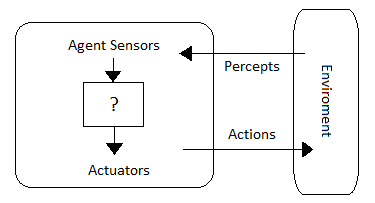
\includegraphics[width=\linewidth, height=3cm, keepaspectratio]{Pictures/ai-ml/agent-env-skeleton.png}
    \caption*{Agents interact with environments through sensors and actuators \cite{aci-1}}
\end{figure}

\begin{enumerate}
    \item An \textbf{agent} is anything that can be viewed as perceiving its \textbf{environment} through \textbf{sensors} and acting upon that environment through \textbf{actuators}.

    \item notion of desirability is captured by a \textbf{performance measure} that evaluates any given sequence of environment states.

    \item As a general rule, it is better to design performance measures according to what one actually wants in the environment, rather than according to how one thinks the agent should behave. 

    \item \textbf{information gathering}: Doing actions in order to modify future percepts
\end{enumerate}


\subsection{Agent}

\begin{enumerate}
    \item Mathematically speaking, we say that an agent’s behavior is described by the \textbf{agent function}\indexlabel{agent function} that maps any given percept sequence to an action.\\
    This an external characterization of the agent.

    \item Internally, the agent function for an artificial agent will be implemented by an \textbf{agent program}\indexlabel{agent program}.

    \item[] The agent function is an abstract mathematical description; the agent program is a concrete implementation, running within some physical system.\\
    SEE: \fullref{Agent Function VS Agent Program}

    \item A \textbf{rational agent} is one that does the right thing—conceptually speaking, every entry in the table for the agent function is filled out correctly. \\
    For each possible percept sequence, a rational agent should select an action that is expected to maximize its performance measure, given the evidence provided by the percept sequence and whatever built-in knowledge the agent has.

    \item An \textbf{omniscient agent} knows the actual outcome of its actions and can act accordingly; but omniscience is impossible in reality. 

    \item Rationality maximizes expected performance, while perfection maximizes actual performance.

    \item To the extent that an agent relies on the prior knowledge of its designer rather than on its own percepts, we say that the agent lacks \textbf{autonomy}.\\
    A rational agent should be autonomous—it should learn what it can to compensate for partial or incorrect prior knowledge. 
\end{enumerate}


\subsection{Environment}

\begin{enumerate}
    \item The environment is the external system or world in which the agent operates. It provides inputs (percepts) to the agent and reacts to the agent's actions. \cite{chatgpt}

    \item The “geography” of the environment is known \textbf{"a priori"} 
\end{enumerate}


\subsection{Sensor (input device) \cite{chatgpt}}

\begin{enumerate}
    \item A sensor is a device that allows an agent to perceive its environment. 
    
    \item It collects information from the environment, such as a camera capturing images or a thermometer measuring temperature.
\end{enumerate}


\subsection{Actuator (output device) \cite{chatgpt}}

\begin{enumerate}
    \item An actuator is a mechanism or device that the agent uses to take physical actions in the environment. 
    
    \item For example, in robotics, motors and servos are actuators that move parts of the robot.
\end{enumerate}


\subsection{Percepts (input)}

\begin{enumerate}
    \item \textbf{percept} refers to the agent’s perceptual inputs at any given instant

    \item \textbf{percept sequence} is the complete history of everything the agent has ever perceived

\end{enumerate}


\subsection{Actions (output)}

\begin{enumerate}
    \item an agent’s choice of action at any given instant can depend on the entire percept sequence observed to date, but not on anything it hasn’t perceived
\end{enumerate}



\section{Task Environment}

\begin{enumerate}
    \item task environments are essentially the “problems” to which rational agents are the “solutions.”

    \item "task environment" means "environment of task" in literal sense, but it actually means "scenario of task" or "task ecosystem"
\end{enumerate}

\subsection{PEAS description of task environment}
\begin{enumerate}
    \item P - Performance
    \item E - Environment
    \item A - Actuators
    \item S - Sensors
\end{enumerate}

Example:
\begin{customTableWrapper}{1.2}
\begin{table}[H]
    \centering
    \begin{tabular}{|l p{10cm}|}
        \hline
        \textbf{Task Environment} & automated taxi \\
        \hline\hline
        
        \textbf{Agent} & Taxi driver \\
        \hline

        \textbf{Performance Measure} & Safe, fast, legal, comfortable trip, maximize profits \\

        \textbf{Environment} & Roads, other traffic, pedestrians, customers \\

        \textbf{Actuators} & Steering, accelerator, brake, signal, horn, display \\

        \textbf{Sensors} & Cameras, sonar, speedometer, GPS, odometer, accelerometer, engine sensors, keyboard \\
        \hline
    \end{tabular}
\end{table}
\end{customTableWrapper}






